\documentclass[tikz,border=7pt]{standalone}
\usepackage{amsmath}
\usetikzlibrary{arrows.meta}
\begin{document}
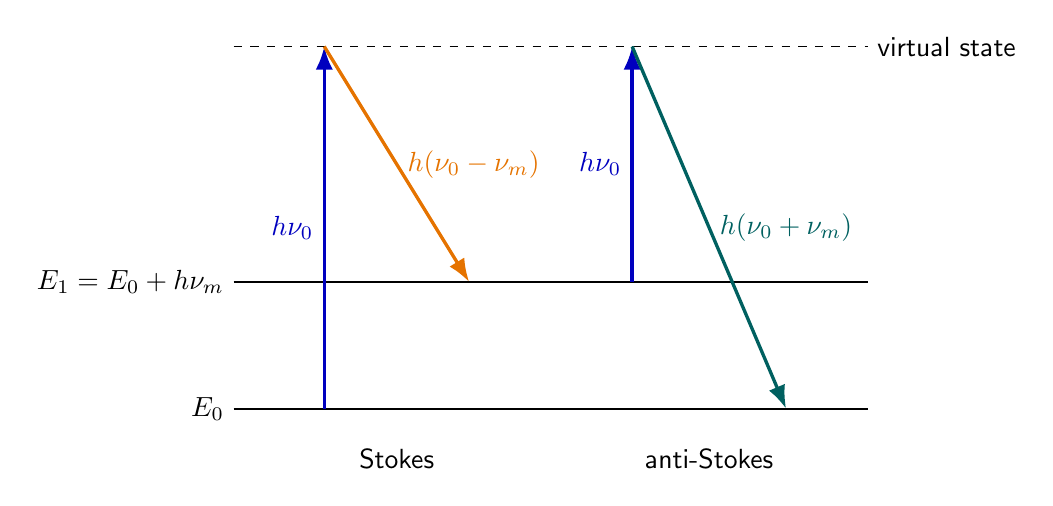
\begin{tikzpicture}[>=Latex,font=\sffamily,x=1.15cm,y=1.15cm]
\foreach \y/\lab in {0/$E_0$,1.4/$E_1=E_0+h\nu_m$}{\draw[thick] (0,\y)--(7,\y);\node[left] at (0,\y){\lab};}
\draw[dashed] (0,4.0)--(7,4.0) node[right]{virtual state};
\draw[->,blue!75!black,very thick] (1,0)--(1,4) node[midway,left]{$h\nu_0$};
\draw[->,orange!90!black,very thick] (1,4)--(2.6,1.4) node[midway,right]{$h(\nu_0-\nu_m)$};
\node at (1.8,-.55){Stokes};
\draw[->,blue!75!black,very thick] (4.4,1.4)--(4.4,4) node[midway,left]{$h\nu_0$};
\draw[->,teal!75!black,very thick] (4.4,4)--(6.1,0) node[midway,right]{$h(\nu_0+\nu_m)$};
\node at (5.25,-.55){anti-Stokes};
\end{tikzpicture}
\end{document}
